\documentclass[MASTER.tex]{subfiles} 
\begin{document} 

%- http://www.appliedmissingdata.com/sample-chapter.pdf
%- http://www.unt.edu/rss/class/Jon/Benchmarks/MissingValueImputation_JDS_Nov2010.pdf
%- http://stats.stackexchange.com/questions/11991/are-misses-in-my-data-distributed-completely-at-random
%- http://www.jstatsoft.org/article/view/v045i07



%- http://www.theanalysisfactor.com/missing-data-mechanism/
%- http://finzi.psych.upenn.edu/library/BaylorEdPsych/html/LittleMCAR.htm
	%------------------------------------------------------%
	% http://www.psychwiki.com/wiki/Analyzing_Data
	% http://www.upa.pdx.edu/IOA/newsom/semclass/ho_missing.pdf
	% http://www.uvm.edu/~dhowell/StatPages/More_Stuff/Missing_Data/Missing.html
	% http://www.uvm.edu/~dhowell/StatPages/More_Stuff/Missing_Data/Missing.html
	% http://www.stat.columbia.edu/~gelman/arm/missing.pdf
	% https://onlinecourses.science.psu.edu/stat505/node/78
	% http://rer.sagepub.com/content/45/4/543.full.pdf
	% http://www.kdnuggets.com/faq/precision-recall.html
	
%========================================================================== %
\begin{frame}

%  Missing Data Leadout
%  NA
%  Complete Cases
%  Types of Missing Data
%  Little MCAR Test
%  Patterns
%  Imputations

\begin{figure}
\centering
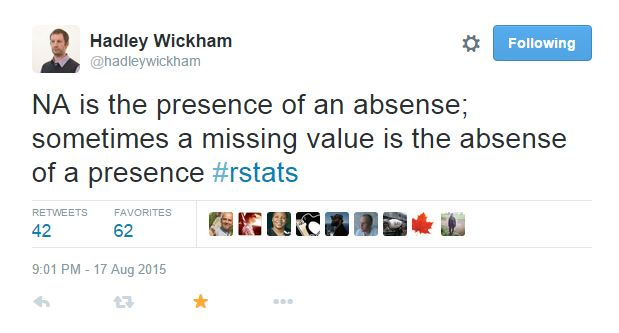
\includegraphics[width=1.1\linewidth]{MissingValues-HWquote}
\end{figure}

\end{frame}
\begin{frame}
	\begin{figure}
\centering

\includegraphics[width=1.1\linewidth]{MissingValues-HWquote2}
\end{figure}

	\end{frame}
%==================================================================== %
\begin{frame}[fragile]
		\frametitle{Missing Data}
		\Large
	\noindent \textbf{Introduction}
		\begin{itemize}
\item 	Missing data is a common problem in all kinds of research. 
\item The way you deal with it depends on how
		much data is missing, the kind of missing data (single items, a full questionnaire, a measurement
		wave), and why it is missing, i.e. the reasons that the data are missing.
\item  Handling missing data is an
		important step in several phases of a scientific study.
		\end{itemize}

		
	\end{frame}
	%====================================================== %
	\begin{frame}
		\Large
		\frametitle{Dealing with Missing Data}
		\begin{itemize}
			\item 		Missing values means reduced sample size and loss of data. 
			%You conduct research to measure empirical reality so missing values thwart the very purpose of research. 
			
			\item 		The less data collected, the less data that can be analyzed, and reducing the data that can be analyzed reduces statistical power, which is the ability to detect real relationships in the data.
			\item  Missing values may also indicate bias in the data. If the missing values are non-random, then the study is not accurately measuring the intended constructs. 
			\item The results of your study may have been different if the missing data was not missing.
		\end{itemize}		
		
	\end{frame}
%========================================= %	
\begin{frame}[fragile]
		\Large
		\frametitle{Missing Values in \texttt{R}}
		\noindent \textbf{The NA Symbol}
		\begin{itemize}
\item In \texttt{R}, missing values are represented by the symbol NA (not available) . 
\item Impossible values (e.g., dividing by zero) are represented by the symbol \texttt{NaN} (not a number). 

\end{itemize}
\end{frame}
%========================================= %	
\begin{frame}[fragile]
	\Large
\noindent \textbf{Excluding Missing Values from Analyses}
Arithmetic functions on missing values yield missing values.
	\begin{framed}
		\begin{verbatim}
x <- c(1,2,NA,3)
mean(x) # returns NA
mean(x, na.rm=TRUE) # returns 2
\end{verbatim}
\end{framed}
\end{frame}
	%========================================= %	
\begin{frame}[fragile]
		\Large
\begin{itemize}
\item The function \texttt{complete.cases()} returns a logical vector indicating which cases are complete.
\end{itemize}		
	\begin{framed}
		\begin{verbatim}
# list rows of data that 
# have missing values 
mydata[!complete.cases(mydata),]
\end{verbatim}
\end{framed}
	\end{frame}
	%========================================= %	
	\begin{frame}[fragile]
		\Large
\begin{itemize}
\item The function \texttt{na.omit()} returns the object with listwise deletion of missing values.
\end{itemize}

\begin{framed}
\begin{verbatim}	
# create new dataset without missing data 
newdata <- na.omit(mydata)
\end{verbatim}
\end{framed}
\end{frame}	
%====================================================== %
\begin{frame}
\Large
\frametitle{Why do missing values occur?}
\begin{itemize}
\item		Missing values are either \textbf{random} or \textbf{non-random}.
		
\item 		Random missing values may occur because the subject inadvertently did not answer some questions. 
\item  The study may be overly complex and/or long, or the subject may be tired and/or not paying attention, and miss the question. 

\item Random missing values may also occur through data entry mistakes.
	\end{itemize}

	\end{frame}
\subfile{MissingData-Types.tex}
	%====================================================== %
	\begin{frame}
		\Large
	\begin{itemize}
	\item 	Non-random missing values may occur because the subject purposefully did not answer some questions.  \item  The question may be confusing, so many subjects do not answer the question. 
	\item Also, the question may not provide appropriate answer choices, such as \textbf{\textit{no opinion}} or \textit{\textbf{not applicable}}, so the subject chooses not to answer the question.
	\end{itemize}
		
	\end{frame}
	%====================================================== %
%	\begin{frame}
%		\Large
%		Also, subjects may be reluctant to answer some questions because of social desirability concerns about the content of the question, such as questions about sensitive topics like Criminal record, addiction issues, personal prejudices etc.
%	\end{frame}

	%====================================================== %
	\begin{frame}
		\Large
		\frametitle{Dealing with Missing Data}
		There are three approaches to dealing with missing data.
		\begin{description}
			\item[ Option 1] Continue With the Incomplete Data
			\item[ Option 2] Casewise deletion
			\item[ Option 3] Imputation
		\end{description}
	\end{frame}
	%====================================================== %
	\begin{frame}
		\Large
		%---------------------------------------------------------------%
		\frametitle{Option 1 : Continue With the Incomplete Data}
		\begin{itemize}
\item The first option is to leave the data as is, with the missing values in place. 
\item This is the most frequent approach, for a few reasons. First, the number of missing values are typically small. Second, missing values are typically non-random. 
\item Third, even if there are a few missing values on individual items, you typically create composites of the items by averaging them together into one new variable, and this composite variable will not have missing values because it is an average of the existing data. 
		\end{itemize}

		
		%However, if you chose this option, you must keep in mind how SPSS will treat the missing values.
		
	\end{frame}
	%====================================================== %
%	\begin{frame}
%		\Large
%		\frametitle{Pairwise Deletions and Listwise Deletion}
%		\noindent \textbf{Listwise Deletion}		\begin{itemize}
%%\item SPSS will not include cases (subjects) that have missing values on the variable(s) under analysis. 
%\item If you are only analyzing one variable, then listwise deletion is simply analyzing the existing data. 
%\item If you are analyzing multiple variables, then listwise deletion removes cases (subjects) if there is a missing value on any of the variables. 
%\item The disadvantage is a loss of data because you are removing all data from subjects who may have answered some of the questions, but not others (e.g., the missing data).
%		\end{itemize}
%
%	\end{frame}
	%====================================================== %
%	\begin{frame}
%		\Large
%		\noindent \textbf{Pairwise Deletion} 
%	\begin{itemize}
%% \item SPSS will include all available data. 
%\item Unlike listwise deletion which removes cases (subjects) that have missing values on any of the variables under analysis, pairwise deletion only removes the specific missing values from the analysis (not the entire case).
%	\end{itemize}
%	\end{frame}
	%====================================================== %
%	\begin{frame}
%		\Large
%		\begin{itemize}
%\item In other words, all available data is included.  - If you are conducting a correlation on multiple variables, then SPSS will conduct the bivariate correlation between all available data points, and ignore only those missing values if they exist on some variables. In this case, pairwise deletion will result in different sample sizes for each correlation. 
%\item Pairwise deletion is useful when sample size is small or missing values are large because there are not many values to begin with, so why omit even more with listwise deletion.
%
%		\end{itemize}
%		\end{frame}
	%====================================================== %
	\begin{frame}
		\Large
		
		\frametitle{Option 2 : Case-Wise Deletion}
		\begin{itemize}
\item The next option is to delete cases with missing values.  
\item For every missing value in the dataset, you can delete the subjects with those missing values. 
\item Thus, you are left with complete data for all subjects.
		\end{itemize}
	
	\end{frame}
	%====================================================== %
	\begin{frame}
		\frametitle{Option 2 : Case-Wise Deletion}
		\Large
		\begin{itemize}
			\item		
		The disadvantage to this approach is you reduce the sample size of your data (sometimes most of it). 
		\item If you have a large dataset, then it may not be a big disadvantage because you have enough subjects even after you delete the cases with missing values.
\end{itemize}	
\end{frame}
	%====================================================== %
	\begin{frame}
	\frametitle{Option 2 : Case-Wise Deletion}
	\Large
		\begin{itemize}
		\item Another disadvantage to this approach is that the subjects with missing values may be different than the subjects without missing values (i.e MNAR), so you have a non-representative sample after removing the cases with missing values.
		\end{itemize}

	\end{frame}

	%====================================================== %
	\begin{frame}
		\frametitle{Option 3 : Imputation}
		\Large
				\begin{itemize}
\item The last option is to replace the missing values, called \textbf{imputation}. 
\item There is little agreement about whether or not to conduct \textbf{imputation}. 
\item There is some agreement, however, in which type of imputation to conduct.  
\item You typically do NOT conduct \textbf{Mean substitution} or \textbf{Regression substitution}.
		\end{itemize}

	\end{frame}
	%====================================================== %
	\begin{frame}
		\frametitle{Option 3 : Imputation}
		\Large
		\begin{itemize}
			\item \textbf{Mean substitution} is replacing the missing value with the mean of the variable.
			\item \textbf{Regression substitution} uses regression analysis to replace the missing value.\\  Regression analysis is designed to predict one variable based upon another variable, so it can be used to predict the missing value based upon the subject’s answer to another variable.
			
		\end{itemize}
		
		The favored type of imputation is replacing the missing values using different estimation methods. % %The \textbf{\textit{Missing Values Analysis}} add-on module in SPSS contains the estimation methods.
		
	\end{frame}
	

	%http://www.upa.pdx.edu/IOA/newsom/semclass/ho_missing.pdf
	
	%------------------------------------------------------%
	
	
	%http://www.uvm.edu/~dhowell/StatPages/More_Stuff/Missing_Data/Missing.html
	
	% http://www.uvm.edu/~dhowell/StatPages/More_Stuff/Missing_Data/Missing.html
	% http://www.stat.columbia.edu/~gelman/arm/missing.pdf
	%---------------------------------------------------------------------------------------------------%
	
\end{document}
